% -----------------------------------------------
\documentclass[aspectratio=169, xcolor={dvipsnames}, xtable]{beamer}
\usetheme{metropolis}

% Inline quotations
\usepackage{csquotes}

% Font rendering
\usepackage{fontspec}

% Colors
\usepackage{xcolor}
\usepackage{colortbl}

% Code listings
\usepackage{listings}

% Math support
\usepackage{amsmath}
\usepackage{amssymb}
\usepackage{amsfonts}
\usepackage{mathtools}
\usepackage{mathpartir}
\usepackage{stmaryrd}
\usepackage{bm}

% Hyperlinks
\usepackage{hyperref}

% Date formatting
\usepackage[UKenglish]{isodate}

% References
\usepackage[style=trad-abbrv, sortcites, backend=biber]{biblatex}
\setbeamertemplate{bibliography item}[text]

\addbibresource{references.bib}

% -----------------------------------------------
\title{Compiling Functional Programs with Holes}
\subtitle{}
\author{Hilbert Chen, Yanjun Chen, \textbf{Eric Zhao} \\\\
Advisor: Cyrus Omar \\
Future of Programming Lab, University of Michigan}
\date{}

% -----------------------------------------------
\begin{document}

% Smol footnotes
\setbeamerfont{footnote}{size=\tiny}


% Use Fira Code for code
\setmonofont[
  Contextuals={Alternate},
  Scale=MatchLowercase
]{Fira Code}

% Hyperlink style
\hypersetup{
    linkcolor=blue,
    filecolor=magenta,
    urlcolor=cyan,
}
\urlstyle{same}

% Piece-wise uncovering of elements in TikZ pictures
\tikzset{
  invisible/.style={opacity=0},
  visible on/.style={alt={#1{}{invisible}}},
  alt/.code args={<#1>#2#3}{%
    \alt<#1>{\pgfkeysalso{#2}}{\pgfkeysalso{#3}} % \pgfkeysalso doesn't change the path
  },
}

% Default listing style
\lstdefinestyle{default}{%
  basicstyle=\ttfamily\footnotesize,
  showspaces=false,
  showstringspaces=false,
  showtabs=false,
  tabsize=1,
  commentstyle=\color{black!60}
}
\lstset{style=default}

\definecolor{lavender}{RGB}{162,85,162}

\newcommand{\SyNEHole}[3]{\ensuremath{\textcolor{lavender}{\bm{\llparenthesis}}#1\textcolor{lavender}{\bm{\rrparenthesis}^{#2}_{#3}}}}
\newcommand{\SyEHole}[2]{\ensuremath{\SyNEHole{}{#1}{#2}}}

\newcommand{\SyTInt}{\ensuremath{\textsf{Int}}}
\newcommand{\SyTBool}{\ensuremath{\textsf{Bool}}}

\newcommand{\SyDArrow}{\ensuremath{~\Rightarrow~}}
\newcommand{\SyNDArrow}{\ensuremath{~\nRightarrow~}}
\newcommand{\SyArrow}{\ensuremath{~\to~}}
\newcommand{\SyBar}{\ensuremath{\vert~}}
\newcommand{\SyColon}{\ensuremath{~\textbf{:}~}}
\newcommand{\SyInn}{\ensuremath{~\textbf{in}~}}
\newcommand{\SyIn}{\ensuremath{\textbf{in}~}}
\newcommand{\SyLet}{\ensuremath{\textbf{let}~}}
\newcommand{\SyWith}{\ensuremath{~\textbf{with}~}}
\newcommand{\SyWrap}{\ensuremath{\textbf{wrap}}}

\newcommand{\SyCastL}{\ensuremath{\langle}}
\newcommand{\SyCastR}{\ensuremath{\rangle}}

\newcommand{\SyPlus}{\ensuremath{+}}
\newcommand{\SyTimes}{\ensuremath{*}}
\newcommand{\SyTrue}{\ensuremath{\textrm{true}}}

\newcommand{\Indent}{\ensuremath{\hspace{10pt}}}

\newcommand{\isConsistent}[2]{\ensuremath{#1 \sim #2}}
\newcommand{\isNotConsistent}[2]{\ensuremath{#1 \nsim #2}}

\newcommand{\CtxVar}{\ensuremath{\Gamma}}
\newcommand{\HoleCtxVar}{\ensuremath{\Delta}}

\newcommand{\hasType}[2]{\ensuremath{#1 : #2}}
\newcommand{\hasTypeCtx}[4]{\ensuremath{#1, ~#2 \vdash \hasType{#3}{#4}}}

\newcommand{\extendCtx}[3]{\ensuremath{#1 ; ~\hasType{#2}{#3}}}

\newcommand{\rulen}[1]{~~\text{(#1)}}
\newcommand{\judgment}[3]{\inferrule{#1}{#2}\rulen{\textsc{#3}}}
\newcommand{\judgbox}[1]{\noindent \fbox{$#1$}}

\newcommand{\pie}[2]{%
  \begin{tikzpicture}
    \draw (0,0) circle (#1); \fill[rotate=90] (#1,0) arc (0:#2:#1) -- (0,0) -- cycle;
  \end{tikzpicture}%
}

\newcommand{\SyReturn}{\ensuremath{\textbf{return}~}}
\newcommand{\SyCaseComplete}{\ensuremath{\textbf{casecomplete}~}}
\newcommand{\SyEmbed}{\ensuremath{\textbf{emb}}}
\newcommand{\SyProj}{\ensuremath{\textbf{proj}}}

\newcommand{\SortNComplete}{\ensuremath{\textsf{Completeness}}}
\newcommand{\SortNCompleteVar}{\ensuremath{k}}
\newcommand{\SortComplete}{\ensuremath{\textsf{}}}
\newcommand{\SortCompleteVar}{\ensuremath{\overline{k}}}
\newcommand{\SortTypCon}{\ensuremath{\textsf{Type}}}
\newcommand{\SortTypConVar}{\ensuremath{\tau}}
\newcommand{\SortTyp}{\ensuremath{\textsf{}}}
\newcommand{\SortTypVar}{\ensuremath{\overline{\tau}}}
\newcommand{\SortComp}{\ensuremath{\textsf{Composite}}}
\newcommand{\SortCompVar}{\ensuremath{c}}
\newcommand{\SortValue}{\ensuremath{\textsf{Value}}}
\newcommand{\SortValueVar}{\ensuremath{v}}
\newcommand{\SortHoleId}{\ensuremath{u}}

\newcommand{\CNC}{\ensuremath{\pie{0.3ex}{360}}}
\newcommand{\CNI}{\ensuremath{\pie{0.3ex}{0}}}
\newcommand{\CII}{\ensuremath{\pie{0.3ex}{180}}}

\newcommand{\TCHole}{\ensuremath{\SyEHole{}{}}}
\newcommand{\TCInt}{\ensuremath{\SyTInt}}
\newcommand{\TCBool}{\ensuremath{\SyTBool}}

\newcommand{\TIntNC}{\ensuremath{\TMk{\TCInt}{\CNC}}}
\newcommand{\TBoolNC}{\ensuremath{\TMk{\TCBool}{\CNC}}}

\newcommand{\TMk}[2]{\ensuremath{#1[#2]}}

\newcommand{\ENumLit}{\ensuremath{\underline{n}}}
\newcommand{\EBoolLit}{\ensuremath{\underline{b}}}
\newcommand{\ELet}[2]{\ensuremath{\SyLet #1 = #2}}
\newcommand{\EIn}{\ensuremath{\SyInn}}
\newcommand{\EInn}[1]{\ensuremath{\SyIn #1}}
\newcommand{\EReturn}[1]{\ensuremath{\SyReturn #1}}
\newcommand{\ECaseCompleteWith}[1]{\ensuremath{\SyCaseComplete #1 \SyWith}}
\newcommand{\ECaseCompleteBranch}[2]{\ensuremath{\SyBar #1 \SyArrow #2}}

\newcommand{\EWrapIntoNI}[1]{\ensuremath{\SyWrap^{\CNI}~ #1}}
\newcommand{\EWrapIntoII}[1]{\ensuremath{\SyWrap^{\CII}~ #1}}
\newcommand{\EEmbedNC}[1]{\ensuremath{\SyEmbed_{\CNC}~ #1}}
\newcommand{\EEmbedNI}[1]{\ensuremath{\SyEmbed_{\CNI}~ #1}}
\newcommand{\EProj}[2]{\ensuremath{\SyProj[#2]~ #1}}

\newcommand{\EPlusNC}[2]{\ensuremath{#1 \SyPlus_{\CNC} #2}}
\newcommand{\EPlusNI}[2]{\ensuremath{#1 \SyPlus_{\CNI} #2}}
\newcommand{\ETimesNC}[2]{\ensuremath{#1 \SyTimes_{\CNC} #2}}
\newcommand{\ETimesNI}[2]{\ensuremath{#1 \SyTimes_{\CNI} #2}}

\newcommand{\ETrue}{\ensuremath{\SyTrue}}
\newcommand{\EEHole}[2]{\ensuremath{\SyEHole{#1}{#2}}}

\newcommand{\EVarNamed}[2]{\ensuremath{t_{#1}^{{\color{gray}#2}}}}

\newcommand{\currenttitle}{}

\maketitle

\renewcommand{\currenttitle}{Context: Hazel}
\begin{frame}{\currenttitle}
  \only<+->{\textbf{Hazel}\footnote{Omar et al. POPL 2017; Omar et al. POPL 2019} is a pure
  functional programming language with \emph{typed holes} and a live programming environment}
  %
  \begin{itemize}
    \item<+-> \emph{Structure editor} that ensures that \emph{all edit states} are well-formed (by
      inserting holes where necessary)
    \item<+-> Semantics provide both static \emph{and dynamic} meaning to all edit states
  \end{itemize}
  %
  \uncover<+->{We can evaluate \emph{incomplete programs}, i.e. programs with holes!}
\end{frame}

\begin{frame}{\currenttitle}
  \only<+->{
    An example Hazel program:

    \begin{center}
      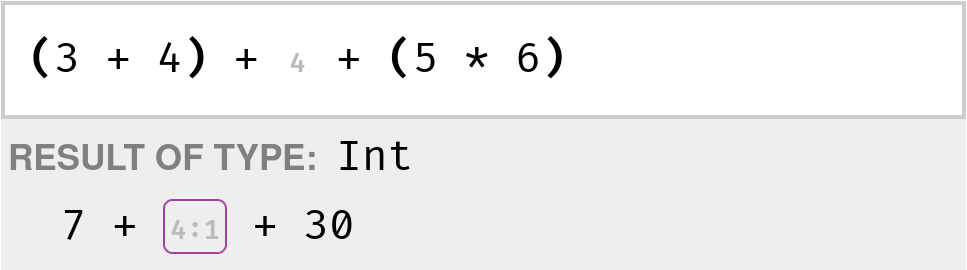
\includegraphics[width=0.5\linewidth]{hazel-demo-code.png}
    \end{center}
  }

  \uncover<+->{Evaluation \emph{continues around} holes and accumulates them into an
  \bf{indeterminate result}.}
\end{frame}

\renewcommand{\currenttitle}{Compiling holes}
\begin{frame}{\currenttitle}
  \only<1->{We explore compiling Hazel to a format that may be executed faster (e.g. for incomplete
  programs with high computation)}
  \begin{itemize}
    \item<2-> Efficient runtime operations and representations of holes
    \item<3-> Integration in a live programming environment
    \item<4-> Compile to WebAssembly\footnote<4->{Haas et al. PLDI 2017} 
      \begin{itemize}
        \item Future integration into existing web-based Hazel UI
        \item For now, via Grain\footnote<3->{Grain (https://grain-lang.org)}, a functional language
          targeting WASM with low-level runtime APIs
      \end{itemize}
  \end{itemize}
  %
  \uncover<5->{More broadly, the design space of compiling holes}
\end{frame}

\renewcommand{\currenttitle}{Compiling holes}
\begin{frame}{\currenttitle}
  Indeterminate results are not values
  \begin{itemize}
    \item Need to build the result tree during runtime
    \item Minimize overhead of dynamically checking if something is a value or indeterminate result
  \end{itemize}
\end{frame}

\renewcommand{\currenttitle}{Compiling holes}
\begin{frame}{\currenttitle}
  Separate memory representation for indeterminate results
  \begin{itemize}
    \item Fitted into existing runtime layouts to take advantage of garbage collector
    \item Fast heap tag check to determine if something is a value or indeterminately incomplete
    \item Runtime library defines how indeterminate results are accumulated
  \end{itemize}
\end{frame}

\renewcommand{\currenttitle}{Completeness analysis}
\begin{frame}{\currenttitle}
  Complete (i.e. no holes) portions of a program should execute using runtime primitives

  \only<+->{Perform static analysis to determine which expressions are guaranteed to be values or
  indeterminate results at runtime}
  \begin{itemize}
    \item<+-> ``Necessarily complete'' $\implies$ value
    \item<+-> ``Necessarily incomplete'' $\implies$ indeterminate result
    \item<+-> ``Indeterminately incomplete'' $\implies$ could be either (dynamic check!)
  \end{itemize}

  \uncover<+->{This is made explicit in the type system of an internal language}
\end{frame}

\begin{frame}{\currenttitle}
  \begin{center}
    \[\begin{array}{rccl}
      \SortNComplete & \SortNCompleteVar & \Coloneqq & \CNC \mid \CNI                                                                              \\
      \SortComplete  & \SortCompleteVar  & \Coloneqq & \SortNCompleteVar \mid \CII                                                                 \\
      \SortTypCon    & \SortTypConVar    & \Coloneqq & \TCHole \mid \TCInt \mid \TCBool \mid \cdots                                                   \\
      \SortTyp       & \SortTypVar       & \Coloneqq & \SortTypConVar[\SortCompleteVar]                                                            \\
      \SortValue       & \SortValueVar       & \Coloneqq & x \mid \EEHole{\SortHoleId}{\sigma}
                                                     \mid \ENumLit \mid \EBoolLit \mid \cdots                                              \\
      \SortComp      & \SortCompVar      & \Coloneqq & \SortValueVar 
                                                     \mid \EPlusNC{\SortValueVar}{\SortValueVar} 
                                                     \mid \EPlusNI{\SortValueVar}{\SortValueVar} \\
                     &                   & \mid         & \EWrapIntoNI{\SortValueVar}
                                                     \mid \EWrapIntoII{\SortValueVar} \\
                     &                   & \mid         & \EEmbedNC{\SortValueVar}
                                                     \mid \EEmbedNI{\SortValueVar}
                                                     \mid \EProj{\SortValueVar}{\SortTypConVar} \\
                     &                   & \mid         & \ECaseCompleteWith{\SortValueVar}
                                                       \ECaseCompleteBranch{x}{\SortCompVar}
                                                      ~\ECaseCompleteBranch{x'}{\SortCompVar} \\
                     &                   & \mid         & \ELet{x}{\SortCompVar} \EIn \SortCompVar \\
                     &                   & \mid         & \cdots
    \end{array}\]
  \end{center}
\end{frame}

\begin{frame}{\currenttitle}
  \begin{mathpar}
    \footnotesize
    \uncover<+->{\judgment{
      \SortHoleId :: \SortTypConVar[\CtxVar'] \in \HoleCtxVar \\
      \hasTypeCtx{\CtxVar}{\HoleCtxVar}{\sigma}{\CtxVar'}
    }{
      \hasTypeCtx{\CtxVar}{\HoleCtxVar}{\EEHole{\SortHoleId}{\sigma}}{\TMk{\SortTypConVar}{\CNI}}
    }{TAEHole}} \and

    \uncover<+->{\judgment{ }{
      \hasTypeCtx{\CtxVar}{\HoleCtxVar}{\ENumLit}{\TIntNC}
    }{TANumLit}} \and

    \uncover<+->{\judgment{
      \hasTypeCtx{\CtxVar}{\HoleCtxVar}{\SortValueVar}{\TMk{\TCInt}{\CNC}} \\
      \hasTypeCtx{\CtxVar}{\HoleCtxVar}{\SortValueVar'}{\TMk{\TCInt}{\CNC}}
    }{
      \hasTypeCtx{\CtxVar}{\HoleCtxVar}{\EPlusNC{\SortValueVar}{\SortValueVar'}}{\TMk{\TCInt}{\CNC}}
    }{TAPlusNC}} \and

    \uncover<+->{\judgment{
      \hasTypeCtx{\CtxVar}{\HoleCtxVar}{\SortValueVar}{\TMk{\TCInt}{\CNI}} \\
      \hasTypeCtx{\CtxVar}{\HoleCtxVar}{\SortValueVar'}{\TMk{\TCInt}{\CNI}}
    }{
      \hasTypeCtx{\CtxVar}{\HoleCtxVar}{\EPlusNC{\SortValueVar}{\SortValueVar'}}{\TMk{\TCInt}{\CNI}}
    }{TAPlusNI}} \and

    \uncover<+->{\judgment{
      \hasTypeCtx{\CtxVar}{\HoleCtxVar}{\SortValueVar}{\TMk{\SortTypConVar}{\CII}} \\\\
      \hasTypeCtx{\extendCtx{\CtxVar}{x}{\TMk{\SortTypConVar}{\CNC}}}{\HoleCtxVar}{\SortCompVar}{\SortTypVar} \\
      \hasTypeCtx{\extendCtx{\CtxVar}{x'}{\TMk{\SortTypConVar}{\CNI}}}{\HoleCtxVar}{\SortCompVar'}{\SortTypVar}
    }{
      \hasTypeCtx{\CtxVar}{\HoleCtxVar}{
        \ECaseCompleteWith{\SortValueVar}
          \ECaseCompleteBranch{x}{\SortCompVar}
          ~\ECaseCompleteBranch{x'}{\SortCompVar'}
        }{\SortTypVar}
    }{TACaseComplete}}
  \end{mathpar}
\end{frame}

\renewcommand{\currenttitle}{Cast handling}
\begin{frame}{\currenttitle}
  \only<+->{For casting we use type-indexed embedding/projections\footnote{New and Ahmed, ICFP 2018}:}
  \begin{itemize}
    \item<+-> To hole type: wrap results in proxies with embedded type information
    \item<+-> Away from hole type: project proxies to target type
    \item<+-> May fail, yielding an indeterminate result of a failed cast
  \end{itemize}
  
  \vspace*{-1.5em}
  \uncover<+->{\begin{mathpar}
    \footnotesize
    \judgment{
      \hasTypeCtx{\CtxVar}{\HoleCtxVar}{\SortValueVar}{\TMk{\SortTypConVar}{\CNC}}
    }{
      \hasTypeCtx{\CtxVar}{\HoleCtxVar}{\EEmbedNC{\SortValueVar}}{\TMk{\TCHole}{\CNI}}
    }{TAEmbedNC} \and

    \judgment{
      \hasTypeCtx{\CtxVar}{\HoleCtxVar}{\SortValueVar}{\TMk{\SortTypConVar}{\CNI}}
    }{
      \hasTypeCtx{\CtxVar}{\HoleCtxVar}{\EEmbedNI{\SortValueVar}}{\TMk{\TCHole}{\CNI}}
    }{TAEmbedNI} \and

    \judgment{
      \hasTypeCtx{\CtxVar}{\HoleCtxVar}{\SortValueVar}{\TMk{\SortTypConVar}{\CNI}}
    }{
      \hasTypeCtx{\CtxVar}{\HoleCtxVar}{\EProj{\SortValueVar}{\SortTypConVar'}}{\TMk{\SortTypConVar'}{\CII}}
    }{TAProj}
  \end{mathpar}}
\end{frame}

\renewcommand{\currenttitle}{Ongoing and future work}
\begin{frame}{\currenttitle}
  \only<+->{We are still exploring options for\ldots}
  \begin{itemize}
    \item<+-> Pattern matching
      \begin{itemize}
        \item Patterns may contain \emph{pattern holes}
      \end{itemize}
    \item<+-> Optimized casting
      \begin{itemize}
        \item More space-efficient casting with the coercion-based approach
      \end{itemize}
    \item<+-> Live environment integration
      \begin{itemize}
        \item Need fast compilation and execution to be worthwhile
        \item Hand-off between evaluator and compiler
        \item Fill-and-resume: fill in a previous compiled and executed result when user fills a
          hole
      \end{itemize}
    \item<+-> Proving the compilation pipeline to be correct
  \end{itemize}
\end{frame}

\section*{Thanks!}

\end{document}
